\section{Messaufbau}


\begin{figure}[H]
    \centering
    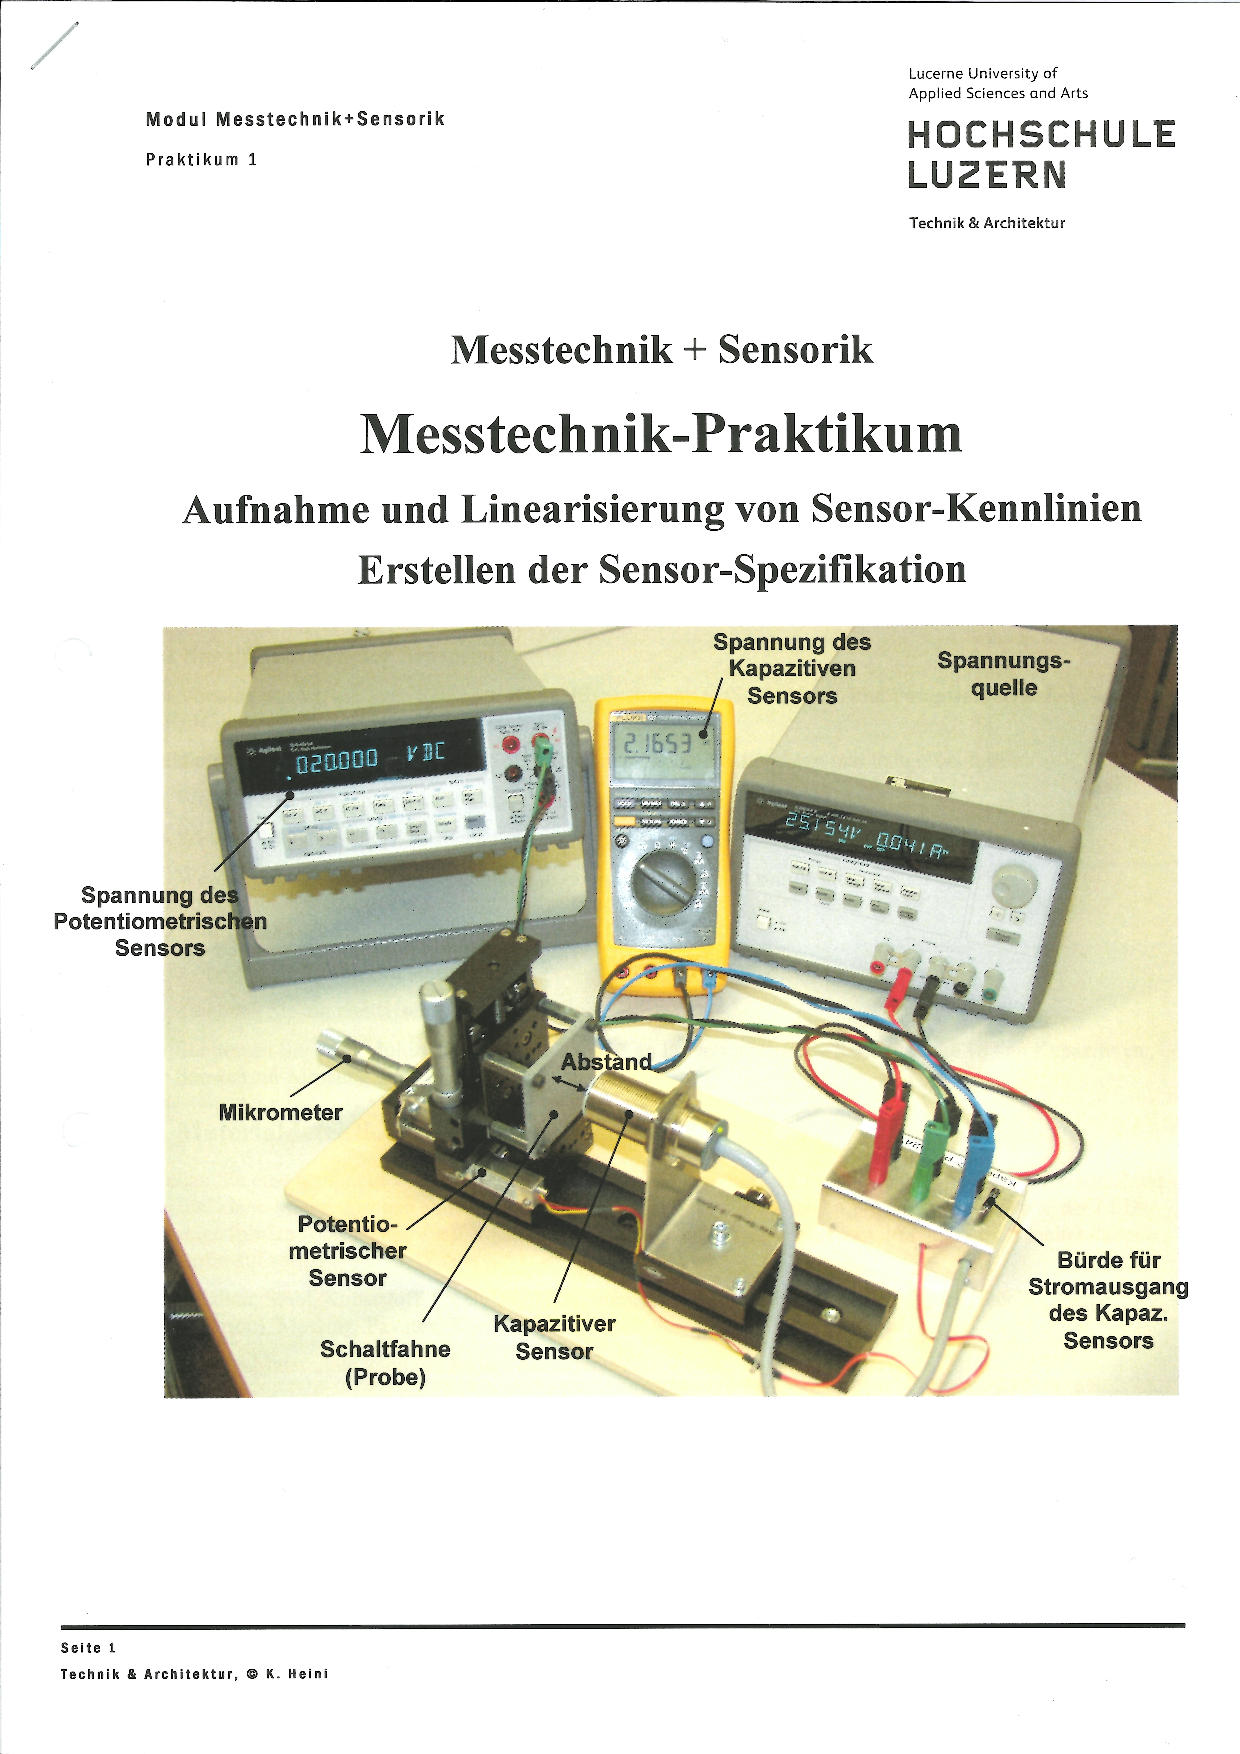
\includegraphics[scale=0.8,trim={0.5cm 6cm 0 10.5cm},clip]{pic/aufbau.pdf}
    \caption{Messaufbau}
    \label{fig:messaufbau}
\end{figure}

Folgende Messgeräte wurden verwendet: \\

\begin{tabular}{ l | l | l}
    \hline
    Hersteller & Typ         & Nummer / Info          \\ \hline
    Agilent    & 34461A..... & nicht vorhanden   \\ \hline
    Burster    & Typ 1164    & Präzisionswiderstand      \\ \hline
    Burster    & Typ 1240-1K & Kalibrationswiderstand \\ \hline
    Kabel    &    -    & kapazitiver Sensor          \\ \hline
    \\ \hline
\end{tabular}


%\subsection{Elektrisches Ersatzschaltbild}
%Ist das Messgerät genug hoch-$\Omega$ oder wird der Spannungsteiler belastet?






\clearpage